\documentclass[a4paper]{article}

\usepackage[spanish]{babel}
\usepackage{graphicx}
\usepackage{amsmath, amssymb}
\usepackage[margin=2cm]{geometry}
\usepackage{fancyhdr}
\usepackage{enumerate}
\usepackage[shortlabels]{enumitem}
\usepackage{parskip}
\usepackage[most]{tcolorbox}
\usepackage[hidelinks]{hyperref}
\usepackage{float}


% cabecera
\pagestyle{fancy}
\fancyhead[l]{Daniel Soto}
\fancyhead[c]{Problemas de Astronomía \#10}
\fancyhead[r]{\today}
\fancyfoot[c]{\thepage}
\renewcommand{\headrulewidth}{0.2pt} % linea horizontal

%% Definicion de comandos para formato de unidades fisicas %%
\newcommand{\m}{\text{m}}
\newcommand{\mm}{\text{mm}}
\newcommand{\cm}{\text{cm}}
\newcommand{\km}{\text{km}}
\newcommand{\s}{\text{s}}
\newcommand{\N}{\text{N}}
\newcommand{\g}{\text{g}}
\newcommand{\kg}{\text{kg}}
\newcommand{\Msolar}{\text{M}_\odot}
\newcommand{\Mterrestre}{\text{\text{M}_\oplus}}
\newcommand{\AU}{\text{AU}}
\newcommand{\ly}{\text{ly}}
\newcommand{\nT}{\text{nT}}
\newcommand{\GeV}{\text{GeV}}
\newcommand{\atomscm}{\text{atoms/cm}^3}
\newcommand{\K}{\text{K}}
\newcommand{\J}{\text{J}}



\newcounter{problema}

\newtcolorbox[use counter=problema]{problema}[1][]{%
	breakable,
    colback=gray!15,
    colframe=gray!60,
    fonttitle=\bfseries,
    title={Problema~\theproblema:},
    boxrule=0.5mm,
    arc=3mm,
    boxsep=5pt,
    left=8pt,
    right=8pt,
    top=6pt,
    bottom=6pt,
    #1
}


\begin{document}

\begin{problema}
\textbf{SDO revela detalles sobre la superficie del Sol:} El 21 de abril de 2010, el Observatorio de Dinámica Solar (SDO) de la NASA publicó sus muy esperadas imágenes de la "Primera Luz" del Sol.

\begin{figure}[H]
        \centering
        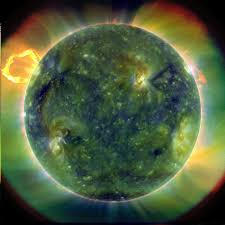
\includegraphics[width=0.5\textwidth]{SDO.jpeg}
        %\caption{}
        \label{fig:1}
\end{figure}

La imagen anterior muestra una imagen de todo el disco, multilongitud de onda, en ultravioleta extremo del Sol, tomada por el SDO el 30 de marzo de 2010. Los colores falsos indican diferentes temperaturas del gas. El negro indica temperaturas muy bajas, cercanas a los 10000 $\K$, cerca de la superficie solar (fotosfera). Los rojos son plasma relativamente frío (un gas compuesto por átomos que han perdido parte de sus electrones) calentado hasta 60000 Kelvin; los azules, verdes y blancos son plasma más caliente, con temperaturas superiores a 1 millón de Kelvin.
\begin{enumerate}

	\item El radio del Sol es de 690000 kilómetros. ¿Cuál es la escala de esta imagen en $\km/\mm$?

	\item ¿Cuáles son las características más pequeñas que puedes encontrar en esta imagen, y qué tamaño tienen en kilómetros, en comparación con la Tierra si el radio de la Tierra es de 6378 kilómetros?

	\item ¿Dónde se ubican en esta imagen el gas más frío (agujeros coronales) y el gas más caliente (llamaradas microscópicas)?
\end{enumerate}
 
\end{problema}

[1] \cite{NASA_SpaceWeatherMath}

\begin{problema}
\textbf{Primer plano de una mancha solar por Hinode:} Después de un lanzamiento exitoso el 22 de septiembre de 2006, el observatorio solar Hinode captó una vista parcial de una gran mancha solar el 4 de noviembre de 2006. 

\begin{figure}[H]
        \centering
        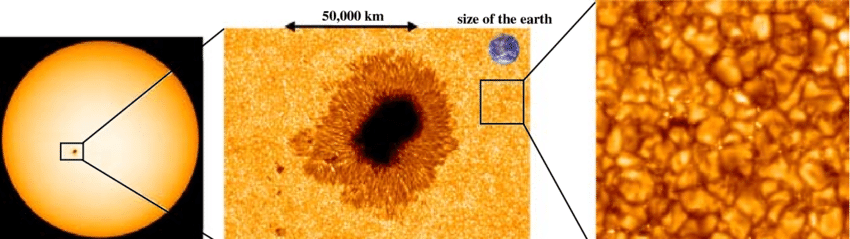
\includegraphics[width=0.7\textwidth]{Sunspot.png}
        %\caption{}
        \label{fig:2}
\end{figure}

Un instrumento llamado Telescopio Óptico Solar (SOT) capturó esta imagen, mostrando detalles de la mancha solar en la superficie solar.

\begin{enumerate}
	\item Basándose en la distancia entre los puntos de las flechas, ¿cuál es la escala de la imagen de la derecha en unidades de kilómetros por milímetro?

	\item ¿Cuál es el tamaño del detalle más pequeño que puedes ver en la imagen?

	\item Comparado con objetos familiares en la superficie de la Tierra, ¿qué tamaño tendría la característica más pequeña en la imagen solar?

	\item La superficie dorada y texturizada es la fotosfera del Sol. La textura se produce por gas caliente que fluye hacia la superficie desde el interior caliente del Sol. Los gases convectivos forman células, llamadas granulaciones, en la superficie, con gas ascendente proveniente del centro de cada célula, hacia los bordes de la célula, donde se enfría y fluye de vuelta hacia capas más profundas. ¿Cuál es el tamaño promedio de una célula de granulación dentro del cuadrado?

	\item Mide varias células de granulación a diferentes distancias del centro de la mancha solar y grafica el tamaño promedio que obtienes en función de la distancia desde el centro de la mancha. ¿Las células de granulación tienen aproximadamente el mismo tamaño cerca de la mancha solar, o tienden a hacerse más grandes o más pequeñas a medida que te acercas a la mancha solar?
\end{enumerate}

\end{problema}
[2] \cite{NASA_SpaceWeatherMath}

\begin{problema}
\textbf{Energía Cinética y Masa de CMEs (Erupciones de Masa Coronal):} 
La energía cinética es la energía que tiene un cuerpo en virtud de su masa y velocidad. Matemáticamente, se expresa como la mitad del producto de la masa del objeto por el cuadrado de su velocidad:

$$E_k = \frac{1}{2}mv^2$$

Entre octubre de 1996 y mayo de 2006, el satélite SOHO detectó y catalogó 11 031 erupciones de masa coronal (CMEs). Hubo suficientes datos disponibles para determinar las propiedades de 2 131 eventos. La siguiente tabla proporciona valores para diez de estas CMEs.

\begin{table}[H]
    \centering
    \begin{tabular}{|c|c|c|c|}
        \hline
        \textbf{Fecha} & \textbf{Velocidad (km/s)} & \textbf{E.C. (Joules)} & \textbf{Masa (kilogramos)} \\
        \hline
        4/8/1996   &             & \( 1.1 \times 10^{20} \) & \( 2.2 \times 10^9 \) \\
        \hline
        8/22/2000  & 388          & \( 1.3 \times 10^{22} \) & \\
        \hline
        6/10/2001  & 731          & \( 8.2 \times 10^{23} \) & \\
        \hline
        1/18/2002  & 64           &                         & \( 2.6 \times 10^{10} \) \\
        \hline
        5/16/2002  & 1,310        &                         & \( 7.8 \times 10^{10} \) \\
        \hline
        10/7/2002  &              & \( 7.8 \times 10^{21} \) & \( 3.0 \times 10^{10} \) \\
        \hline
        1/24/2003  & 387          & \( 9.1 \times 10^{18} \) & \\
        \hline
        10/31/2003 & 2,198        & \( 1.6 \times 10^{24} \) & \\
        \hline
        11/2/2003  &              & \( 9.3 \times 10^{25} \) & \( 4.5 \times 10^{13} \) \\
        \hline
        11/10/2004 & 3,387        &                         & \( 9.6 \times 10^{12} \) \\
        \hline
    \end{tabular}
    \caption{Valores medidos de diez CMEs observadas por el satélite SOHO.}
    \label{tab:CME_data}
\end{table}


\begin{enumerate}
	\item Complete la tabla determinando el valor de las entradas faltantes usando la fórmula de la Energía Cinética.

	\item ¿Cuál es el rango mínimo y máximo de las energías cinéticas observadas para las 10 CMEs? La bomba de hidrógeno más grande jamás probada fue la Bomba del Zar en 1961 y fue equivalente a 50 megatones de TNT. Tuvo un rendimiento de $ 5 \times 10^{23} \J$. ¿Cuál es el rendimiento equivalente de la CME más grande en megatones y en “Bombas del Zar”?

	\item ¿Cuáles son las masas equivalentes de las CMEs más pequeña y más grande en toneladas métricas?

	\item Compare la masa de la CME más grande con la masa de una montaña pequeña. Suponga que la montaña puede representarse como un cono con un volumen dado por $\frac{1}{3} \pi r^2 h $, donde $r$ es el radio de la base y $h$ es la altura en metros, y suponga que la densidad de la roca es $3 \g / \cm ^3$.
\end{enumerate}

\end{problema}
[30] \cite{NASA_SpaceWeatherMath}

\bibliographystyle{plainurl}
\bibliography{bibliografia} % Nombre del .bib

\end{document}
